\documentclass[output=paper]{langsci/langscibook} 
\title{Tone features revisited: Evidence from Seenku (Mande, Burkina Faso)} 
\author{%
Laura McPherson \affiliation{Dartmouth College} 
}
% \chapterDOI{} %will be filled in at production


\abstract{
Recently, authors such as \citet{Hyman10b} and \citet{Clementsetal10} have argued that African tone is better modeled with tonal primitives (e.g.\ H, M, L) than with tonal features. This paper reopens the question with novel data from Seenku, a four-tone Mande language of Burkina Faso (eL, L, H, eH). I argue that the features [$\pm$upper, $\pm$raised] provide a unified analysis of several tonal phenomena, including plural formation, tonal neutralizations, and verbal alternations. First, I argue that plural formation is a case of featural affixation, with a plural suffix [+raised] deriving [-upper,+raised] L from singular eL, while underlying [+upper,-raised] H shifts to eH. In terms of tonotactics, the two middle tones are treated differently in nouns: [+upper,-raised] is not allowed word-finally and is always followed by eL, while derived [-upper,+raised] is allowed. Further evidence for tone features is found in the verbal domain. First, the distinction between eH and H in verbs is often neutralized, to eH for transitive verbs and H for intransitive verbs. I analyze these neutralizations as default [+raised] assignment to underlying [+upper] verbs in the transitive and [-raised] assignment in the intransitive. In the perfective, eH-toned transitive verbs are realized as H while eL-toned verbs remain unchanged. A featural account derives this result with the affixation of perfective [-raised]. Finally, complicated argument-head tonal alternations may be more naturally explained under a featural approach. In sum, this paper presents a case where tonal features show an analytic advantage over tonal primitives, suggesting that the debate is not yet over.
}

\maketitle
\begin{document}

 \section{Introduction}
 
 Segments are widely accepted in phonology to consist of phonological features. These features encode parameters such as place ([labial], [coronal], [dorsal]), voicing ([voice]), nasality ([nasal]), or manner ([sonorant], [continuant], [delayed release]). For tone, the situation is much less clear. Unlike segments, tone relies on only one phonetic parameter, f0 (barring secondary features like phonation), which is inherently scalar rather than binary.
 
Nevertheless, numerous feature systems for tone have been proposed in the literature. \citet{Wang67} proposed a seven feature system for tone, including three height features ([high], [central], [mid]), and four contour features ([contour], [rising], [falling], [convex]). Later systems abandoned featural specification for contour tones, opting to view contours as sequences of tone levels instead. The most widely accepted systems take four level tones as the base, which can be achieved with two binary features. \citet{Yip80} proposed a so-called Register feature [$\pm$upper], dividing tonal space into two halves further subdivided by a second feature (sometimes called a Tone feature) [$\pm$high]. This latter feature was renamed [raised] by \citet{Pulleyblank86}. Other authors such as \citet{Clements83}, \citet{Snider90}, and \citet{Hyman93} use unary features, [h/l] for Register and [H/L] for Tone, but the resulting systems function in largely the same way.

Despite numerous proposals for both African languages and tone languages elsewhere, recent work has cast doubt on the use of features for tone. \citet{Hyman10b}, for instance, points out problems for M tones in featural systems, including featural ambiguity in a three-tone language and the lack of a natural class for M tones in a four-tone language. \citet{Clementsetal10} echo these criticisms, pointing to the lack of clear natural classes defined by tone features and to the lack of support for assimilation or dissimilation patterns driven by tonal features. For these reasons, both sets of authors suggest that at least African tone is better modeled in autosegmental terms with simple levels (L, M, H, etc.).

This paper has two main goals. The first is to describe the tone system of southern Seenku, a relatively undescribed Mande language of Burkina Faso. The second is to reopen the debate on the featural underpinnings of tone. I will argue that a two-feature system aids in the analysis of Seenku, drawing evidence from plural formation, transitive/intransitive tonal neutralization, perfective formation, and argument-head tonal alternations found in inalienable possession and certain O+V constructions.

The paper is structured as follows: \sectref{sec:mcpherson:SecBackground} provides background information on Seenku and data sources, and in \sectref{sec:mcpherson:SecTone}, I give a brief description of Seenku lexical tone. The core arguments for tonal features are given in \sectref{sec:mcpherson:SecEvidence}, where I address plural formation (\sectref{sec:mcpherson:SecPl}), transitive/intransitive tonal neutralization (\sectref{sec:mcpherson:SecTransitive}), perfective formation (\sectref{sec:mcpherson:SecPFV}), and argument-head tonal alternations (\sectref{sec:mcpherson:SecAlternations}). \sectref{sec:mcpherson:SecAlternatives} considers alternative analyses and \sectref{sec:mcpherson:SecConclusion} concludes.





\section{Language and data}\label{sec:mcpherson:SecBackground}


Seenku (ISO 639-3 [sos]) is a Mande language of the Samogho subfamily spoken in southwestern Burkina Faso. It has two main dialects, each named after the main village where the dialect is spoken: northern Seenku (Timiku, literally `language of Karangasso') with 5,000 speakers and southern Seenku (Gbeneku, literally `language of Bouend\'e') with 12,000 speakers \citep{Ethnologue}. The former was the subject of Prost's (\citeyear{Prost71}) {\it \'El\'ements de Sembla}, a short grammar sketch and lexicon, but the latter has received very little scholarly attention apart from Congo's (\citeyear{Congo13}) Master's Thesis on aspects of the phonology. Since 2013, I have undertaken fieldwork on the southern dialect; all data in this paper are drawn from my field notes.

Like most Mande languages, Seenku shows S Aux O V X word order, where X can be occupied by an indirect object, PP, negation, or adverb. Morphologically, it is largely isolating.

\section{Sketch of the tone system}\label{sec:mcpherson:SecTone}

Seenku is a four-tone language, with tonal primitives e(xtra)L, L, H, and e(xtra)H, though with a few exceptions the underlying tonal inventory can be reduced to three (eL, H, eH); as we will see below, L is commonly the result of plural formation, where it contrasts with singular eL, but is rarely found lexically. Minimal sets contrasting even these three underlying levels are remarkably difficult to find, given an apparent tonotactic restriction on H in word-final position in nouns and many tonal neutralizations found in verbs (see \sectref{sec:mcpherson:SecTransitive} and \sectref{sec:mcpherson:SecPFV}). In pronouns, we find the following (near) minimal pairs for eL vs.\ H and H vs.\ eH, respectively:\footnote{Tonal transcription represents eL with double grave $<$\textipa{\H*a}$>$, L with grave $<$\textipa{\`a}$>$, H with acute $<$\textipa{\'a}$>$, and eH with double acute $<$\textipa{\H{a}}$>$. Tone marking for the whole syllable is otherwise only marked on the first vowel, e.g.\ {\it \textipa{b\H*EE}} `pig' is a long level eL. The most common contour tones are HeL and eLeH, represented by circumflex $<$\textipa{\^a}$>$ and hacek $<$\textipa{\v{a}}$>$, respectively. The less common falling contour eHeL is represented by umlaut $<$\textipa{\"a}$>$. All of these contour tones are likewise marked on the first vowel only, representing the fact that tone is a property of the syllable rather than the mora, and to maintain identity in tone marking between short and long vowels. All other contour tones are only found through processes of vowel coalescence, and in this case only, each component of the contour is marked on one half of the long vowel, e.g.\ HeH $<$\textipa{\'a\H{a}}$>$.}

\ea\label{ex:mcpherson:1}
\ea\label{ex:mcpherson:1a} {\textipa{\H*a}} `3\textsc{sg}' \\
{\textipa{\'a}} `2\textsc{sg}' \\
\ex\label{ex:mcpherson:1b} {\textipa{m\'o}} `1\textsc{sg}' \\
{\textipa{m\H{{\i}}}} `1\textsc{pl}' \\
\z
\z

If we include the repair for noun-final H, i.e.\ epenthesis of eL, the following (near) minimal sets can be identified:\footnote{In these examples, the $<$n$>$ in parentheses represents a floating nasal, usually unpronounced in isolation but realized on the following word in connected speech (either by nasalizing a sonorant or prenasalizing a stop).}

\ea\label{ex:mcpherson:2} {\it Tonal minimal sets contrasting eL, H, and eH} \\
\begin{tabular}[t]{llll} 
   & {eL} & {H(eL)} & {eH} \\
  a. & {\textipa{ky\H*E(n)}} & {\textipa{ky\^E(n)}} & {\textipa{k\H{E}}} \\
   & `peanut' & `breast' & `fat' \\
   & & & \\
  b. & {\textipa{ts\H*{u}}} & {\textipa{ts\^{u}}} & {\textipa{s\H{u}}} \\
   & `thatch' & `hippo' & `antelope' \\  
\end{tabular} 
\z

Underlying L is limited in the current dataset to one numeral, {\it \textipa{n\`O}} `five', and a couple of adverbs, {\it \textipa{k\`Or\`O}} `yesterday' and {\it \textipa{m\`aa}} `again'. Given the limited nature of numeral and adverbial vocabulary, minimal pairs are not available, but L forms a near minimal pair with eL in numerals: {\it \textipa{n\`O}} `five' vs.\ {\it \textipa{n\H*aa}} `four', and the f0 of L on `five' is lower than that of H on {\it \textipa{s\'oen}} `one' when pronounced side-by-side, showing that these two middle tones are indeed phonetically distinct.

Contour tones are very common in Seenku, particularly HeL (illustrated above) and eLeH, found on both heavy and light syllables. This distribution suggests that the tone-bearing unit (TBU) in Seenku is the syllable rather than the mora. An example of a minimal pair contrasting HeL and eLeH is given in \REF{ex:mcpherson:3}:

\ea\label{ex:mcpherson:3} {\textipa{k\^{\~u}\~{\i}}}  `{n\'er\'e} seeds' \\
{\textipa{k\v{\~u}\~{\i}}} `grass sp.' \\
\z

Of these, HeL is the more common contour, found on all syntactic categories; eLeH, in contrast, is particularly common on auxiliaries and adjectives, the latter of which may be grammatically assigned.

The other attested underlying contour is the tritone sequence eLHeL, as in {\it \textipa{d\H*{a}\^a}} `basket hanger'.

Other contours are created morphologically or phonologically, as illustrated in the following examples:

\ea\label{ex:mcpherson:4} {\it Other contour tones and how they are created} \\
\begin{tabular}[t]{llll} 
  {Tone} & {Example} & {Gloss} & {Created by...} \\
  eHeL & {\textipa{n\"{\i}O}} & `has eaten' & Perfect formation \\
  eLeHeL & {\textipa{n\H*{a}\"a}} & `has come' & Perfect formation \\
  HeH & {\textipa{m\'o\H{o}}} & `1\textsc{sg} past' & Past tense formation \\
 HL &  {\textipa{m\'o\`o}} & `1\textsc{sg} genitive' & Genitive formation \\
 eLH & {\textipa{\H*E\'E}} & `3\textsc{sg} genitive' & Genitive formation \\
\end{tabular}
\z


In terms of tone rules, Seenku displays downstep and contour tone simplification, though the domains of these processes and their potential implications for a system of tone features are still under investigation.


\section{Evidence for tone features}\label{sec:mcpherson:SecEvidence}

I propose that tone in Seenku is characterized by the following binary features, using the \citet{Pulleyblank86} feature system:

\ea\label{ex:mcpherson:5} {\it Seenku tone features} \\
\begin{tabular}[t]{|l|c|c|c|c|} \hline
   & eL & L & H & eH \\ \hline
  {[}upper{]} & - & - & + & + \\ \hline
  {[}raised{]} & - & + & - & + \\ \hline
\end{tabular}
\z

The two binary features produce four potential tone levels, all of which are represented in Seenku.\footnote{In the early stages of work, I analyzed the language as a three-tone language, which meant there was ambiguity in the featural specification of the M tone. Nevertheless, differing tonotactic restrictions for erstwhile ``lexical M'' (now H) vs.\ the ``derived M" (now L) supported this four-way featural distinction. Further fieldwork revealed that the two supposedly M tones are in fact phonetically distinct, with the tone derived by plural formation (L) lower than that found underlyingly (H). The discovery of a small number of underlying L tones corroborate the decision to treat Seenku as a four-tone language, despite the majority of lexical contrasts being created with only three levels. In other words, it is thanks to a featural analysis that I became attuned to the possibility of four distinct levels.} As stated above, L is seldom part of an underlying specification and is instead usually derived by the addition of grammatical tone features (featural affixes).

Evidence for the utility of tone features over tonal primitives is drawn from four sources: plural formation, transitive/intransitive verb tone, perfective formation, and tonal interactions between pronominal arguments of nouns and verbs (inalienable possession and O+V constructions). This featural specification for Seenku tone responds to some of the criticisms of tone features, including providing evidence for natural classes and for assimilation and dissimilation patterns.

\subsection{Plural formation}\label{sec:mcpherson:SecPl}

The first piece of evidence for tone features in Seenku comes from nominal plural formation. Here, we see a tone raising process (in addition to vocalic changes that I will not address here), raising eL to L and H to eH; underlying eH in the singular remains eH in the plural, since there are no further tone levels to raise to. For example:

\ea\label{ex:mcpherson:6} {\it Plural tone raising} \\
\begin{tabular}[t]{lllll} 
  a. & eL & $\rightarrow$ & L & \\
  & {\textipa{b\H*EE}} & $\rightarrow$ & {\textipa{b\`EE}} & `pig(s)' \\
  & & & & \\
 b. & H(eL) & $\rightarrow$ & eH & \\
  & {\textipa{b\^{\i}}} & $\rightarrow$ & {\textipa{b\H{{\i}}}} & `goat(s)' \\
 & & & & \\
 c. & eH & $\rightarrow$ & eH & \\
 & {\textipa{s\H{u}}} & $\rightarrow$ & {\textipa{s\H{u}i}} & `antelope(s)' \\
\end{tabular}
\z

I argue that tone raising is driven by a featural affix [+raised] (\citealt{McCarthy83,Lieber87,Wiese94,Akinlabi96,Wolf07}, etc.). The addition of [+raised] to an eL tone ([-upper, -raised]) yields L ([-upper, +raised]). The addition of [+raised] to H ([+upper, -raised]) yields eH ([+upper, +raised]). Finally, the addition of [+raised] to eH tone yields no audible difference, since it is already specified as [+raised]. In short, between the singular and the plural, all four possible tonal specifications are attested.

In tonally complex nouns, only the final tone is altered in the plural, suggesting that the plural [+raised] is a suffix. We see this effect in \REF{ex:mcpherson:7a}, where the final eH absorbs [+raised], leaving the preceding eL unaffected, and in \REF{ex:mcpherson:7b}, where H(eL) raises to eH without effecting the preceding eL in the contour tone:

\ea\label{ex:mcpherson:7} 
\ea\label{ex:mcpherson:7a} {\textipa{j\H*oNw\H{a}}} $\rightarrow$ {\textipa{j\H*oNw\H{E}}} `cat(s)' \\
\ex\label{ex:mcpherson:7b} {\textipa{d\H*a\^a}} $\rightarrow$ {\textipa{d\H*E\H{E}}} `basket hanger(s)' \\
\z
\z

Looking at \REF{ex:mcpherson:7b}, we can see that the feature [+raised] targets H of the tritone eLHeL contour, not eL. This fact is explained if the underlying form is eLH, with the final eL tone added only if plural formation fails to apply. As mentioned in the last section, there is a systematic absence of level H-toned singular nouns in the lexicon:

\ea\label{ex:mcpherson:8} {\it Singular level-tone melodies} \\
\begin{tabular}[t]{llll} 
  & Singular & Plural & Gloss \\
  eL & {\textipa{b\H*EE}} & {\textipa{b\`EE} }& `pig(s)' \\
  H & -- & -- & -- \\
  eH & {\textipa{s\H{u}}} & {\textipa{s\H{u}i}} & `antelope(s)' \\
\end{tabular}
\z

Instead, we find an abundance of HeL contours that become eH in the plural, just as we would expect of a H tone. Examples include:

\ea\label{ex:mcpherson:9} {\it /H/ singular $\rightarrow$ eH plural} \\
\begin{tabular}[t]{lll}
  {\textipa{b\^{\i}}} & {\textipa{b\H{{\i}}}} & `goat(s)' \\
  {\textipa{k\^a}} & {\textipa{k\H{E}}} & `yam(s)' \\
  {\textipa{s\^a(n)}} & {\textipa{s\H{\~E}}} & `rabbit(s)' \\
 {\textipa{g\^OO}} & {\textipa{g\H{O}EE}} & `wood(s)' \\
\end{tabular}  
\z

If eL were part of the underlying representation, then [+raised] would dock to eL, creating HL (e.g.\ {\it \textipa{b\^{\i}}} $\rightarrow$ *{\it \textipa{b\'{\i}\`{}}} `goat(s)').\footnote{HL is never found on a light syllable in Seenku, so no single diacritic is employed to represent it, the circumflex already being used to represent HeL.} This supports an underlying representation /b\'{\i}/, which fills in the systematic gap in singular level tone melodies. Anytime a H tone finds itself in noun-final position, an eL tone is epenthesized as a repair.\footnote{This is either a case of lexical class-specific tonotactics or eL is itself morphological, perhaps encoding singular (though not on eH nouns). I leave this question to future work.} If we assume morphology occurs before phonology, then the plural of H nouns would carry a [+raised] feature that alleviates the need for such an epenthetic eL:

\ea\label{ex:mcpherson:10} \begin{tabular}[t]{llll}
UR & /b\'{\i}$_{\text{sg}}$/ & /b\'{\i}$_{\text{pl}}$/ & \\
Morphology & --- & b\H{\i} & (Addition of [+raised]) \\
Phonotactics & b\^{\i} & --- & \\
SR & [b\^{\i}] & [b\H{\i}] \\
\end{tabular}
\z 

From a constraint-based perspective, *[+upper, -raised]\# would be satisfied in the plural by docking the [+raised] feature and deriving an eH tone, whereas in the singular where no such feature is available, eL epenthesis is the optimal strategy. In contrast, all other tones (eL, L, eH) are level, showing that the phonotactic ban is specifically on the featural specification [+upper, -raised]. 

In sum, plural formation provides evidence for all four tone levels in Seenku, motivated by a single featural affix [+raised].

\subsection{Transitive and intransitive verbal tone}\label{sec:mcpherson:SecTransitive}

The next piece of evidence for features comes from transitive and intransitive verbal tone. On the surface, most verb stems show only a two-way tone contrast, with neutralization of eH and H (though as we will see later, there is a contrast between these two underlyingly).\footnote{Recent fieldwork has unearthed some irregular verbs that do not follow these tonal patterns, including a few eH-toned intransitives, but the majority of verbs do undergo the neutralizations described here.} For transitive verbs, eH and H verb stems neutralize to eH tone, as highlighted in \tabref{tab:mcpherson:1}, with a dummy 3\textsc{sg} object {\it \textipa{\H*a}}.

\begin{table}
\begin{tabularx}{\textwidth}{XXX}
\lsptoprule
Underlying tone & Surface form & Gloss \\
\midrule
eL & \textipa{\H*a s\H*{\~a}} & `buy it' \\
& \textipa{\H*a gy\H*{\~O}} & `grill it' \\
& \textipa{\H*a f\H*O} & `uproot it' \\ & & \\
H & \textbf{\textipa{\H*a k\H{\~u}\~O}} & `bite it' \\
& \textbf{\textipa{\H*a s\H{O}O}} & `sell it' \\
& \textbf{\textipa{\H*a g\H{a}a}} & `pull it' \\ & & \\
eH & \textbf{\textipa{\H*a b\H{\~a}}} & `hit it' \\
& \textbf{\textipa{\H*a dz\H{\~i}}} & `put it' \\
& \textbf{\textipa{\H*a n\H{i}O}} & `eat it' \\
\lspbottomrule
\end{tabularx}
\caption{Transitive verb stems}
\label{tab:mcpherson:1}
\end{table}

Both a lexically H-toned stem like /\textipa{s\'OO}/ `sell' and a lexically eH-toned stem like /\textipa{n\H{\i}O}/ `eat' have eH tone on the surface in constructions where verbal tone is not perturbed by either aspect (see \sectref{sec:mcpherson:SecPFV}) or the presence of an object in the irrealis mood (see \sectref{sec:mcpherson:SecAlternations}), namely the progressive and the immediate past, to be expanded upon below.

For intransitive verbs, eH and H verb stems neutralize to H. However, since the underlying distinction between the two only emerges in the presence of a direct object, it is impossible to determine the underlying tone of intransitive verbs in most cases. \REF{ex:mcpherson:12} gives surface forms only:

\ea\label{ex:mcpherson:12} {\it Intransitive verb stems} \\
\begin{tabular}[t]{lll} 
  & Surface form & Gloss \\
 a. eL & {\textipa{k\H*a}} & `go' \\
  & {\textipa{n\H*a}} & `come' \\
  & {\textipa{k\H*{\i}}} & `die' \\
  & {\textipa{kw\H*aa}} & `farm' \\
 b. H & {\textipa{s\'O}} & `arrive' \\
  & {\textipa{ts\'{\~{\i}}}} & `jump' \\
  & {\textipa{s\'u}} & `get up' \\
  & {\textipa{gy\'OO}} & `return' \\
\end{tabular}
\z

The neutralization of eH and H is a dynamic process that results in alternations. For instance, an ambivalent stem {\it \textipa{gy@ra}} `spill' surfaces as {\it \textipa{gy\H{@}r\H{a}}} when used transitively and {\it \textipa{gy\'@r\'a}} when used intransitively. eL-toned verb stems, on the other hand, always surface with eL. Thus, intransitive {\it \textipa{kw\H*aa}} `farm' is still L-toned {\it \textipa{kw\H*a}} when used transitively.\footnote{The vowel length distinction may be due to an assimilated antipassive suffix in the intransitive form.}

I analyze these patterns as the result of morphological neutralization rules targeting [+upper] tones and shifting their registers to either [+raised] for transitive or [-raised] for intransitive verbs:

\ea\label{ex:mcpherson:13} 
\ea\label{ex:mcpherson:13a} {[}+upper] $\rightarrow$ [+raised] when V$_{\text{transitive}}$ \\
\ex\label{ex:mcpherson:13b} {[}+upper] $\rightarrow$ [-raised] when V$_{\text{intransitive}}$ \\ 
\z
\z

For \REF{ex:mcpherson:13a}, the change to [+raised] in [+upper, +raised] eH verbs is vacuous, since they already carry this specification, while the change to [+raised] in [+upper, -raised] H verbs results in a [+upper, +raised] eH tone. Similarly, for \REF{ex:mcpherson:13b}, the change to [-raised] in [+upper, -raised] H verbs is vacuous, but this same change in [+upper, +raised] eH verbs results in [+upper, -raised] H tone. In both cases, the tonal distinction is neutralized. We know that these neutralizations are the result of more restricted rules and not general floating featural morphemes (e.g.\ [+raised] for transitive, [-raised] for intransitive), since the concatenation of [+raised] with an eL verb in the transitive would raise it to L, a change we do not see.

These featural alternations are most likely related to another tonal change we see in the same realis verb forms: In the periphrastic progressive and immediate past, both of which employ the verb stem followed by the postposition {\it \textipa{nE}}, transitive verbs are followed by an eH tone and intransitive verbs are followed by an eL tone. This tone is most often realized solely on the postposition, leaving transitive verbs followed by eH-toned {\it \textipa{n\H{E}}} and intransitive verbs by eL-toned {\it \textipa{n\H*E}}, but intransitive verb stems with a long vowel allow the eL tone to dock, creating a HeL contour on H-toned stems.\footnote{Presumably, the same docking principles would hold true for transitive verbs as well, but the only audible contour that could be created is an eLeH rising tone, and Seenku displays progressive tonal absorption \citep{HymanSchuh74} when a rising tone is followed by an eH tone. This results in simplification back to eL. Evidence that a rising tone is in fact created on eL-toned transitive verbs can be found in the xylophone surrogate language \citep{McPherson16}, where contour simplification is not encoded; musicians play these verbs as rising tones.} For example:

\ea\label{ex:mcpherson:14} {\it Addition of transitive eH and intransitive eL in postpositional forms} \\
\begin{tabular}[t]{lll}
  a. & {Transitive} &  \\
   & {\textipa{\H*a s\H{O}O}} {\textipa{n\H{E}}} & `sell it' \\
   & {\textipa{\H*a s\H*{\~a} n\H{E}}} & `buy it' \\
   & {\textipa{\H*a kp\H*{\~O}\~O} \textipa{n\H{E}}} & `sew it' \\
   & & \\
  b. & {Intransitive} & \\ 
   & {\textipa{k\H*a n\H*E}} & `go' \\
   & {\textipa{s\'a n\H*E}} & `cry' \\
   & {\textipa{gy\^OO} \textipa{n\H*E}} & `return' \\
\end{tabular}
\z

While it is tempting to view the neutralizations as the synchronic result of partial assimilation to the added tone, this analysis is not supported by the data. First, we might expect under this view that eL-toned transitive verb stems might also raise, which they do not; explanations along the line of parasitic harmony \citep{ColeTrigo88} would hold only of transitive verbs (where H raises to adjacent eH), and not of intransitive verbs where it is the maximally different tone (eH) that lowers. Second, and more importantly, certain idiosyncratic verbs like {\it \textipa{N\'a\H{a} n\H{E}}} `yawn' display a HeH contour on the surface before an eH-toned postposition, showing that there is no reason such contours could not be created by the addition of eH to H-toned transitive verbs. In other words, raising of H to eH before another eH is not automatic. Instead, I argue that the tonal neutralizations shown above may be the grammaticized result of phonetic raising or lowering due to the following tone but cannot be analyzed purely on these grounds from a synchronic perspective.

Summarizing this section, the use of tonal features allows us to clearly capture patterns of neutralization in two ways. First, the feature [+upper] defines a natural class of tones in Seenku, namely eH and H, that is affected by the rules of neutralization. Second, the neutralization itself can be explained in featural terms as the change to [+raised] in transitive verbs and to [-raised] in intransitive verbs.


\subsection{Perfective formation}\label{sec:mcpherson:SecPFV}

We find another case of featural affixation in the perfective, though unlike the plural, its effects are only audible in one type of verb, namely transitive eH-toned verbs. In the transitive, we see a lowering of surface eH-toned verb stems to H; eL-toned verb stems show no change:

\ea\label{ex:mcpherson:15} {\it Perfective forms of transitive verbs} \\
\begin{tabular}[t]{llll}
  & Progressive & Perfective & Gloss \\
 a. eH & {\textipa{\H*a s\H{O}O} \textipa{n\H{E}}} & {\textipa{\H*a s\'OO}} & `sell it' \\
 & {\textipa{\H*a n\H{\i}O} \textipa{n\H{E}}} & {\textipa{\H*a n\'{\i}O}} & `eat it' \\
  & {\textipa{\H*a b\H{\~a}} \textipa{n\H{E}}} & {\textipa{\H*a b\'{\~a}}} & `hit it' \\
 b. L & {\textipa{\H*a s\H*{\~a}} \textipa{n\H{E}}} & {\textipa{\H*a s\H*{\~a}}} & `buy it' \\
 & {\textipa{\H*a gy\H*{\~O}} \textipa{n\H{E}}} & {\textipa{\H*a gy\H*{\~O}}} & `grill it' \\
 & {\textipa{\H*a f\H*O} \textipa{n\H{E}}} & {\textipa{\H*a f\H*O}} & `uproot it' \\
\end{tabular}
\z

Intransitive verbs, like eL transitive verbs, show no tonal change in the perfective (apart from the last case, where the absence of the eL tone and postposition allows the verb stem `return' to surface as level H):

\ea\label{ex:mcpherson:16} {\it Perfective forms of intransitive verbs} \\
\begin{tabular}[t]{llll} 
  & Progressive & Perfective & Gloss \\
 a. L & {\textipa{k\H*a n\H*E}} & {\textipa{k\H*a}} & `go' \\
  & {\textipa{n\H*a n\H*E}} & {\textipa{n\H*a}} & `come' \\
  & {\textipa{k\H*i n\H*E}} & {\textipa{k\H*i}} & `die' \\
  & {\textipa{kw\H*aa n\H*E}} & {\textipa{kw\H*aa}} & `farm' \\
 b. H & {\textipa{s\'O} \textipa{n\H*E}} &  {\textipa{s\'O}} & `arrive' \\
  & {\textipa{ts\'{\~{\i}} n\H*E}} & {\textipa{ts\'{\~{\i}}}}  & `jump' \\
  & {\textipa{s\'u n\H*E}} & {\textipa{s\'u}} & `get up' \\
  & {\textipa{gy\^OO} \textipa{n\H*E}} & {\textipa{gy\'OO}} & `return' \\
\end{tabular}
\z

I analyze the perfective as a featural affix [-raised]. Added to [+upper, +raised] eH, this affix derives [+upper, -raised] H. Added to [+upper, -raised] H or [-upper, -raised] eL, it has no audible effect. Because of this, it is indeterminable whether perfective formation applies before or after tonal neutralizations; the resulting forms would be the same either way. 

Thus, the existence of featural affixes in Seenku is corroborated by data from the perfective. Without tone features, we would have to propose an arbitrary rule of eH-tone lowering in the perfective, whereas the affixation of [-raised] explains both the cases where the affix is audible and those where it is not.

\subsection{Alternations with pronominal internal arguments}\label{sec:mcpherson:SecAlternations}

The final argument for tone features is more speculative and is made based on a series of complicated tonal alternations that arise between either a verbal or nominal head and its internal argument (direct object or possessor) when that argument is pronominal. The contexts in which these alternations take place are summarized in \REF{ex:mcpherson:17}:

\ea\label{ex:mcpherson:17} 
\ea\label{ex:mcpherson:17a} A pronominally possessed {\bf inalienable} noun. \\
\ex\label{ex:mcpherson:17b} A transitive verb in {\bf irrealis mood} (future, imperative, habitual) with a pronominal object. \\
\z
\z

When the verb is realis (including when it is perfective), it does not interact tonally with the object.

Before we turn to the alternations, the inventory of Seenku pronouns is summarized in \tabref{tab:mcpherson:2}.

\begin{table}
\begin{tabularx}{\textwidth}{XXX} \lsptoprule 
   Person & Singular & Plural \\ \midrule
  1 & {\textipa{\'n}/\textipa{m\'o}} & {\textipa{m\H{\i}}} \\ 
  2 & {\textipa{\'a (w\'o)}} & {\textipa{\'{\i} (y\'o kw\H{E})}} \\ 
  3 & {\textipa{\H*a w\H*o}} & {\textipa{\H*{\i}}/\textipa{kw\H{E}}} \\ \lspbottomrule
\end{tabularx}
\caption{Seenku pronouns}
\label{tab:mcpherson:2}
\end{table} 

Where there are slashes in \tabref{tab:mcpherson:2}, the form on the left is the basic (unfocused) form and the form on the right is the focused form; similarly, elements in parentheses are added after pronouns when they are focused. As we can see, all three basic tones (eL, H, eH) are attested on pronouns, while L is absent.

When a noun or verb takes a pronoun as its argument, it follows the pronoun and displays tonal alternations depending on both its own underlying tone and on the tone of the pronoun. It is here that we see the three-way tonal contrast on verb stems emerge despite its neutralization in other contexts. \tabref{tab:mcpherson:3} summarizes the alternations, which are the same for both nouns and verbs. The body of the table displays the resulting tonal form of the head noun or verb based on its underlying form (top row) following pronouns of varying tonal forms (leftmost column).

\begin{table}
\begin{tabularx}{\textwidth}{X|XXX} 
\lsptoprule
Final tone & \multicolumn{3}{c}{Underlying tone of head} \\
of pronoun & eL & H & eH \\ \midrule
eL & eL & eL & H \\
H & eH & eL & eL \\
eH & eH & eH & eH \\
\lspbottomrule
\end{tabularx}
\caption{Summary of tonal alternations}
\label{tab:mcpherson:3}
\end{table}

One pattern is clear and straightforward: all head tones are neutralized to eH tone after an eH-final pronoun (1\textsc{pl}, focused 2\textsc{pl} and 3\textsc{pl}). The pattern with eL-final pronouns (3\textsc{sg}, unfocused 3\textsc{pl}) is likewise fairly consistent: it triggers lowering on the head, with eH becoming H, H becoming eL, and eL remaining eL (the opposite pattern of that seen in the plural). The pattern with H-final pronouns (1\textsc{sg}, 2\textsc{sg}, unfocused 2\textsc{pl}) is the most challenging: there is polarity of underlying eL and eH tone, and H lowers to eL. 

How can tone features help us make sense of this situation?

First, it is important to note that after non-pronominal (nominal) arguments, the tone of the head always takes on the final tone of its argument; that is, it is always neutralizing.\footnote{This is reminiscent of tonal compounding processes elsewhere in Mande, e.g.\ {\it compacit\'e tonale} in Bambara \citep{Creissels78,Creissels88,Creissels92,Dumestre84,Green10}, tonal compounding in Susu \citep{Gregoire78,Greenetal13}, as well as in other Western Mande languages \citep{deZeeuw79}.} We can see this in \REF{ex:mcpherson:20}, where the same verb {\it \textipa{s\H*{\~a}}} `buy' takes an eL-, L-, and eH-toned object:

\ea\label{ex:mcpherson:20} 
\ea\label{ex:mcpherson:20a} {\textipa{b\H*EE} \textipa{s\H*{\~a}}} `buy a pig!' \\
\ex\label{ex:mcpherson:20b} {\textipa{b\`EE} \textipa{s\`{\~a}}} `buy pigs!' \\
\ex\label{ex:mcpherson:20c} {\textipa{b\H{\i}} \textipa{s\H{\~a}}} `buy goats!' \\
\z
\z

The examples in \REF{ex:mcpherson:21} show the neutralization of verbal lexical tone after a eL-toned object:

\ea\label{ex:mcpherson:21} 
\ea\label{ex:mcpherson:21a} /eL/ {\textipa{b\H*EE} \textipa{s\H*{\~a}}} `buy a pig!' \\
\ex\label{ex:mcpherson:21b} /H/ {\textipa{b\H*EE} \textipa{s\H*OO}} `sell a pig!' \\
\ex\label{ex:mcpherson:21c} /eH/ {\textipa{b\H*EE} \textipa{b\H*{\~a}}} `hit a pig!' \\
\z
\z

Multiple analyses are possible for the distinction between nouns and pronouns as the argument of the head. One possibility relies on underspecification: tone spreading or copying only takes place after fully specified tones. Under this approach, eH-toned pronouns would be necessarily fully specified as [+upper, +raised], whereas eL- and H-toned pronouns would be missing one of the tonal features. The problem with this approach is that in cases with complex arguments (compound nouns or possessive phrases as the object of a verb), the verb undergoes the same tonal alternations as it would after a pronoun, despite the complex argument arguably having full tonal specification. A second possibility is that differences result from phrasing or domain assignment: arguments and heads seek to form a unified, possibly binary domain, in which the initial element is tonally dominant. Nouns are prosodically stronger than pronouns and are able to fully fill this role, while pronouns cannot overpower the tone of the head. The exception is with eH-toned pronouns, which tend to be CV in shape rather than V or N (impossible syllable shapes in nouns); the combination of the ``strong tone'' eH and their nominal shape allows them to behave like a regular noun. The similarities in tonal effects between pronominal and complex arguments would come from the fact that in both cases the argument is a non-ideal tonal head: in the former case, it is too light, and in the latter case, it is too heavy.

I will leave these explanations for future work and offer here only some preliminary thoughts on why we find the particular tonal alternations described in \tabref{tab:mcpherson:3} as opposed to any others. I will show that tone features may indeed hold the key.

Whether we fully specify eL-toned pronouns as [-upper, -raised] or underspecify them as [-raised] alone, alternations with these pronouns follow straightforwardly from the spread of the [-raised] feature:

\ea\label{ex:mcpherson:22} {\it Example of [-raised] spreading} \\
% 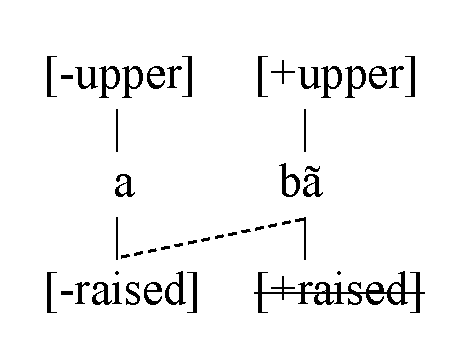
\includegraphics[scale=.5]{figures/Lspread2.eps} \\
\begin{tikzpicture}
\node at (0,0) (-upper) {\strut [-upper]};
\node [below=\baselineskip of -upper] (a) {\strut a};
\node [below=\baselineskip of a] (-raised) {\strut [-raised]};
\node [right= of -upper] (+upper) {\strut [+upper]};
\node [below=\baselineskip of +upper] (ba) {\strut b\~{a}};
\node [below=\baselineskip of ba] (+raised) {\strut\st{[+raised]}};
\draw (-upper) -- (a) -- (-raised);
\draw (+upper) -- (ba) -- (+raised);
\draw [dashed] (ba.south) -- (-raised.north);
\node [below=.5\baselineskip of -raised] (hit) {\strut `hit}; \node [below=.5\baselineskip of +raised] (him) {\strut him!'};
\end{tikzpicture}
\z
\todo[inline] {I aligned the translation with the example figure. OK?}

The pronoun and the verb here are linked with the feature [-raised], which causes the verb to lower from eH to H. 

H-toned pronouns are trickier, since they neither consistently raise nor consistently lower the head. However, I argue that these alternations, too, can be understood as a preference for spreading [-raised] of [+upper, -raised] combined with an OCP effect against adjacent H tones. When a H-toned pronoun precedes an eH head, [-raised] spreads. However, this creates a sequence of two H tones; to resolve this sequence, [+upper] on the head dissimilates to [-upper], yielding an eL tone:

\ea\label{ex:mcpherson:23} {\it Example of [-raised] spreading from H to eH} \\
% 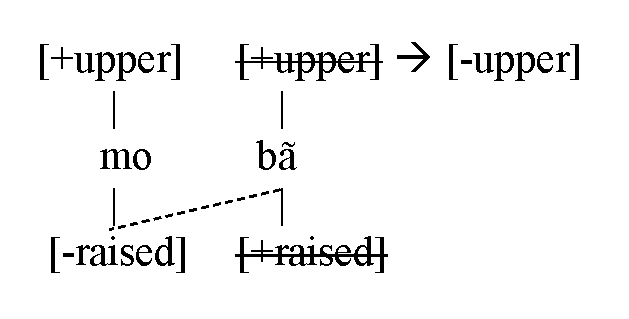
\includegraphics[scale=.55]{figures/MspreadH.eps} \\
\begin{tikzpicture}
\node at (0,0) (-upper) {\strut [+upper]};
\node [below=\baselineskip of -upper] (mo) {\strut mo};
\node [below=\baselineskip of mo] (-raised) {\strut [-raised]};
\node [right= of -upper] (+upper) {\strut\st{[+upper]}}; \node [right= of +upper] (-upp) {\strut [-upper]}; \draw[->,thick] (+upper) -- (-upp);
\node [below=\baselineskip of +upper] (ba) {\strut b\~{a}};
\node [below=\baselineskip of ba] (+raised) {\strut\st{[+raised]}};
\draw (-upper) -- (mo) -- (-raised);
\draw (+upper) -- (ba) -- (+raised);
\draw [dashed] (ba.south) -- (-raised.north);
\node [below=.5\baselineskip of -raised] (hit) {\strut `hit}; \node [below=.5\baselineskip of +raised] (me) {\strut me!'};
\end{tikzpicture}
\z
\todo[inline]{this example has changed. Do you approve?}

With an underlyingly H-toned head, the OCP restriction comes into effect right away, triggering the same repair of dissimilating [+upper] to [-upper]. This results in an eL tone once again:

\ea\label{ex:mcpherson:24} {\it Example of [+upper] dissimilating in a sequence of two Hs} \\
% 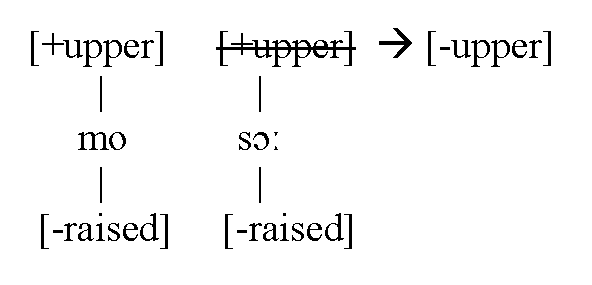
\includegraphics[scale=.6]{figures/MspreadM.eps} \\
\begin{tikzpicture}
\node at (0,0) (-upper) {\strut [+upper]};
\node [below=\baselineskip of -upper] (mo) {\strut mo};
\node [below=\baselineskip of mo] (-raised) {\strut [-raised]};
\node [right= of -upper] (+upper) {\strut\st{[+upper]}}; \node [right= of +upper] (-upp) {\strut [-upper]}; \draw[->,thick] (+upper) -- (-upp);
\node [below=\baselineskip of +upper] (ba) {\strut sɔ\textlengthmark};
\node [below=\baselineskip of ba] (+raised) {\strut [-raised]};
\draw (-upper) -- (mo) -- (-raised);
\draw (+upper) -- (ba) -- (+raised);
\node [below=.5\baselineskip of -raised] (sell) {\strut `sell}; \node [below=.5\baselineskip of +raised] (me) {\strut me!'};
\end{tikzpicture}
\z

Taking H to be a middle tone in Seenku, this kind of M-tone dissimilation has support in other African languages, such as Leggbo \citep{Paster03}. Alternatively, the dissimilation could be driven by an OCP constraint (e.g.\ \citealt{McCarthy86}) on [+upper] rather than on the sequence of two Hs specifically. However, a similar dissimilation pattern is arguably at work with eL-toned heads. Here, rather than spreading [-raised] onto a tone already designated as [-raised], the non-homophonous [+upper] spreads instead. This creates once again a sequence of two H tones, and here it is [-raised] that dissimilates on the head to [+raised], creating an eH tone:

\ea\label{ex:mcpherson:25} {\it example of [+upper] spreading from H to eL} \\
% 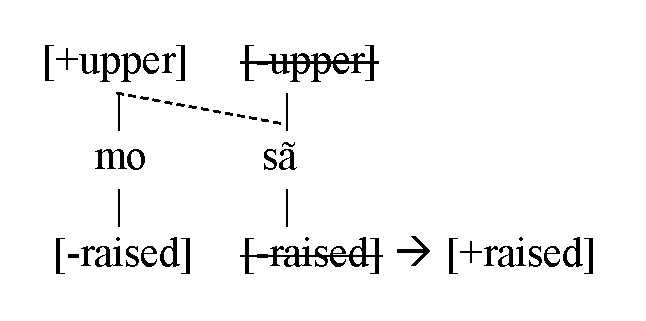
\includegraphics[scale=.58]{figures/MspreadL.eps} \\
\begin{tikzpicture}
\node at (0,0) (-upper) {\strut [+upper]};
\node [below=\baselineskip of -upper] (mo) {\strut mo};
\node [below=\baselineskip of mo] (-raised) {\strut [-raised]};
\node [right= of -upper] (+upper) {\strut\st{[-upper]}};
\node [below=\baselineskip of +upper] (ba) {\strut s\~{a}};
\node [below=\baselineskip of ba] (+raised) {\strut\st{[-raised]}}; \node [right= of +raised] (+rais) {\strut [+raised]}; \draw[->,thick] (+raised) -- (+rais);
\draw (-upper) -- (mo) -- (-raised);
\draw (+upper) -- (ba) -- (+raised);
\draw [dashed] (-upper.south) -- (ba.north);
\node [below=.5\baselineskip of -raised] (buy) {\strut `buy}; \node [below=.5\baselineskip of +raised] (me) {\strut me!'};
\end{tikzpicture}\z

These results can be unified by the following informally conceived constraints: 1. The argument and the head should be linked tonally, preferably by [-raised]. 2. This linking should be of a non-homophonous tonal feature. 3. Two H tones may not follow one another (or, there is an OCP constraint on [+upper] and [-raised]). 

Pronoun-head configurations are still under investigation in Seenku, but the use of tone features brings us closer to understanding how we can get cases of partial assimilation (only one feature spreads rather than both) and why we get the particular changes that we do. We further find promising cases of featural dissimilation of [+upper] and [-raised], driven either by the features themselves or by the larger tonal complex (H) in which they are found.



\section{Feature-less alternatives}\label{sec:mcpherson:SecAlternatives}

If \citet{Hyman10b} and \citet{Clementsetal10} are correct that tone should not be modeled with features, then alternative approaches must be found for Seenku. In this section, I briefly consider two possibilities, showing where each is successful and where it falls short.

\subsection{Tonal primitives (eL, L, H, eH)}\label{sec:mcpherson:5.1}

Under this approach, tones are indivisible elements. The tonal neutralizations found in transitive and intransitive verb tone could be explained by differential phonotactics or reduced inventories: transitive verbs only allow eH and eL and intransitive verbs only allow H and eL.

However, the other tonal effects do not emerge as easily. First, we might try to explain the tone raising chain shift in the plural with the affixation of eH, where eL+eH yields L and H+eH yields eH, but seeing as the language allows contour tones, there is no principled reason why these tone mergers should take place; the situation is the same for the lowering effect of the perfective. Second, there is no natural explanation for the restricted nature of L. Under a two feature system, four categories are automatically available, and L is derived naturally by grammatically manipulating these features. Under a tonal primitive analysis, this fourth category would need to be specifically posited and then restricted to (mostly) derived environments. Finally, the tonal alternations found between pronouns and their lexical head would require even more stipulated tone rules without the availability of features.


\subsection{Scalar tone}\label{sec:mcpherson:5.2}

A more promising alternative is the use of a scale for tone, shown in \REF{ex:mcpherson:26}:

\ea\label{ex:mcpherson:26} {\it Seenku scalar tone} \\
\begin{tabular}[t]{llll}
  eL &  L & H & eH \\
  1 & 2 & 3 & 4 \\
\end{tabular}
\z

Raising in plural formation would be easily accounted for in this system by a rule of [+1] (1 $\rightarrow$ 2, 3 $\rightarrow$ 4). Perfective formation would be a rule of [-1], but only in transitive verbs and only after the neutralization rules that raise /H/ to eH. As above, this would require that we stipulate reduced tonal inventories for transitive and intransitive verbs. The lowering effect with eL-toned pronouns, however, would be problematic, since a rule of [-1] would create a L tone from a H tone rather than the attested eL. Further, the tonal effects with H-toned pronouns do not follow naturally, since tone level 1 raises to 4, while both 4 and 3 lower to 1.

Thus, like the tonal primitive approach, this approach faces a number of difficulties that are more elegantly solved under the featural account.


\section{Conclusion}\label{sec:mcpherson:SecConclusion}

To sum up, tone features have been rejected based in part on the following criticisms:

\begin{enumerate}
  \item No evidence for tonal natural classes, as in segmental phonology. 
  \item No evidence for assimilation or dissimilation patterns.
  \item They give rise to ambiguity in M tones for three-tone languages.
  \item Everyone employs them differently; there is no accepted standard.
\end{enumerate}

In this paper, I have argued that some of these criticisms need to be reconsidered. First and foremost, the existence of tonal features allows us to posit featural affixes for tone, which allow for the elegant analysis of a number of phenomena in Seenku. The data thus far give evidence of a {[+raised]} featural affix marking plural, a {[-raised]} featural affix marking perfective, and possible [+raised] and [-raised] marking transitive and intransitive, respectively, on underlying [+upper] verb stems. On this point, the existence of a tone rule or featural affix targeting only [+upper] verb stems responds directly to criticsm 1: Seenku provides evidence for tonal natural classes.\footnote{It is interesting to note that all of the featural affixation required for Seenku involves the feature [raised]. In this light, we might take [raised] to be the register feature, as in Snider (\citeyear{Snider90}; \citeyear{Snider98}), and thus think of Seenku morphological processes as manipulating register. Future work will explore this topic further, focusing on the relationship between downstep (an attested process in Seenku phonology) and the featurally defined tones presented in this paper.}

In response to criticism 2, we may find evidence for both assimilations and dissimilations in pronoun/head alternations. Specifically, there may be an OCP effect of [-raised] and [+upper] sequences, triggering dissimilation on the second feature, while feature spreading of [-raised] could be viewed as an assimilatory process.

Criticism 3 is a bit difficult to assess, given Seenku's four-tone nature. As I have shown, however, the vast majority of lexical contrasts are produced with only three tones, with the second ``middle tone" restricted to contexts derived by manipulating tone features of the other three. I take this as evidence that the availability of four categories under a feature system may actually be a boon not only for analysis but also for the development of a four-tone system out of what was presumably a system with fewer contrasts historically (as evidenced by related Mande languages).

Finally, criticism 4 is a valid point: there is no accepted standard for tonal features or their geometry. However, I do not view this as reason to abandon the hypothesis. Either we simply have not examined enough languages yet in light of tonal features to reach a consensus, or, as \citet{Odden10} argues, feature systems need not be phonetically-grounded and universal. They may be deduced by speakers from the learning data, leading to different systems and analyses in different cases. 

If languages like Seenku continue to respond to these criticisms, then it may not be time to close the book on tonal features just yet.

\section*{Acknowledgments}

I would like to thank the editors of this volume as well as two anonymous reviewers for their helpful feedback on this paper. Further thanks to Stephanie Shih, Keith Snider, and the audience at ACAL 46. I gratefully acknowledge my Seenku language consultants, Sy Cl\'ement Traor\'e, Gni Emma Traor\'e, and Gni Fatou Traor\'e, and the financial support of NSF Grant BCS-1263150 and the Dartmouth College Office of the Provost, without whom this work would not be possible.

\printbibliography[heading=subbibliography,notkeyword=this]

\end{document}